\subsection{Programming Model}

The key-value store accelerator is controlled through the RISC-V RoCC
co-processor interface. This interface allows the CPU to interact with the
accelerator by sending it custom instructions. A RoCC instruction is encoded
as follows.

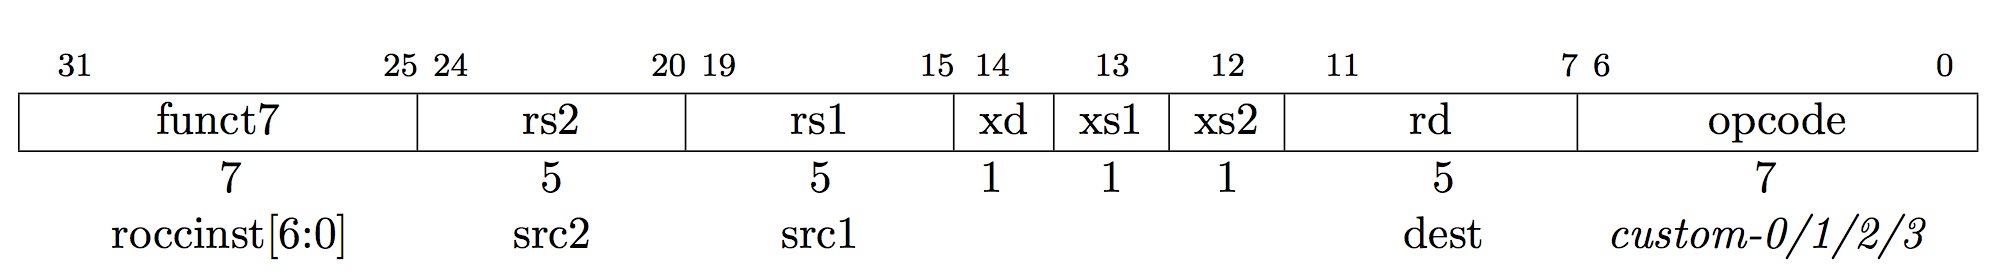
\includegraphics[width=0.9\linewidth]{../../img/rocc-encoding.png}

We use only the custom0 instruction, so the opcode is always 0001011.
The rd, rs1, and rs2 fields refer to the address of the destination and
first and second operand registers, respectively. The xd, xs1, and xs2 bits
are set if the register is actually used by the instruction, and clear
otherwise. The funct7 section of the instruction is essentially a secondary
opcode. Our accelerator specifies seven instructions, which are distinguished
by the value of the funct7 field.

\begin{tabular}{|c|l|c|}
    \hline
    funct7 & name & xd, xs1, xs2 \\
    \hline
    0 & Switch Mode & 000 \\
    1 & Delete Key & 111 \\
    2 & Reserve Key & 111 \\
    3 & Associate Address & 011 \\
    4 & Associate Length & 011 \\
    5 & Write Value & 011 \\
    6 & Reset Counts & 000 \\
    \hline
\end{tabular}

The "switch mode" instruction changes the accelerator to either write mode or
read mode, depending on the value of the rs1 field. Read mode is rs1=0,
write mode is rs1=1. The accelerator must be in read mode in order to serve
responses to the traffic manager, but must be in write mode in order to run
any of the other instructions.

The "delete key" instruction removes a key-value association from the
accelerator. For this instruction, the first source register contains the
starting address of the key in memory, and the second source register contains
the length of the key. The hash value that the key was deleted from is placed
in the destination register. If the key was not present in the accelerator,
the special value 0xffffff is placed in the destination register.

The "reserve key" instruction adds a key to the accelerator. As in the
"delete key" instruction, the first source register is the starting address
of the key. The second register serves a dual function. The lowest eight
bits of the register value are treated as the length of the key (keys are
limited to 255 bytes in size), and the six bits above are treated as the
"weight". The reserve key instruction will replace an existing key if the
weight provided is greater than the access count stored for that key in the
accelerator. The hash value at which the key was placed is returned in the
destination register. If the accelerator could not find a place to put the key,
the special value 0xffffff is placed in the destination register.

The "associate address" instruction associates an address in the value RAM
with a hash value. The hash value is placed in the first source register and
the address is placed in the second source register.

The "associate length" instruction associates the length of a value with a hash
value. The first source register holds the hash value and the second source
register holds the length.

The "write value" instruction transfers a value from the processor's memory to
the accelerator's value memory. The first source register holds the hash value
and the second source register holds the starting address in the CPU memory.
The starting destination address and length must be set earlier using the
"associate address" and "associate length" instructions. The accelerator makes
no attempt to stop one value from overwriting another. Software running on the
CPU performs slab allocation of the value SRAM to ensure that the values do
not overlap.

The "reset counts" instructions resets the access counts for all hash values
to zero. The access counts are saturating 6-bit counters. Every time the key
at a given hash value is accessed, the counter is incremented (unless it is
already saturated). Resetting the counts to zero every once in a while ensures
that old keys which were once popular but no longer are can be evicted from
the accelerator.

To set a key on the accelerator and then activate the accelerator, we would
write a program like the following pseudocode.

\begin{verbatim}
function setKey(key, value, weight)
    // set to write mode
    setMode(1)
    len_weight = len(key) | (weight << 8)
    hash = reserveKey(key, len_weight)
    if hash == 0xffffff then
        raise exception
    // allocate some space on the value SRAM
    // (done in software)
    addr = sramAlloc(len(value))
    // write the value to the accelerator
    assocAddr(hash, addr)
    assocLen(hash, len(value))
    writeVal(hash, value)
    // switch back to read mode
    setMode(0)
\end{verbatim}
